\subsection*{Overview}
Within the retrain.py script \textcite{retrainInception}, as mentioned in
previous experiments, there are various parameters that can be set and changed.
I tested out a few combinations of the parameters to see if I could increase the
test accuracy of the model.

\subsection*{Network Architecture}
The Inception V3 architecture was used for this model.

\subsection*{Dataset}
The Food-101 dataset \textcite{food101} with additional classes, as per
experiment 6, was used for this model.

\subsection*{Libraries}
The libraries in use for this experiment are tensorflow and numpy.

\subsection*{Script}
Script as seen in experiment 5 but with some additions to the command as seen
below:

\begin{lstlisting}
python tensorflow/examples/image_retraining/retrain.py \ --image_dir
~/dataset_directory \ --how_many_training_steps 4000 \ --learning_rate 0.01 \
--testing_percentage 10 \ --validation_percentage 10
\end{lstlisting}

Some further parameters could be set such as:
\begin{itemize}
	\item{--flip\_left\_right}
	\item{--random\_crop}
	\item{--random\_scale}
	\item{--random\_brightness}
\end{itemize}

\begin{figure}
    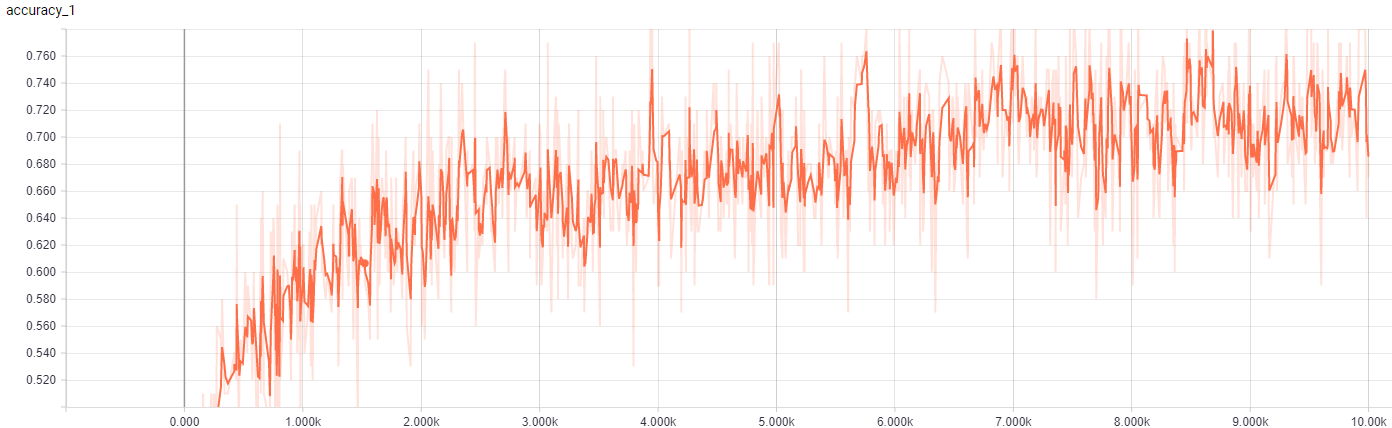
\includegraphics[scale=0.5]{model_test}
     \caption{Graph of accuracy of the test dataset during training}
     \label{fig:model_train_test}
\end{figure}

\begin{figure}
    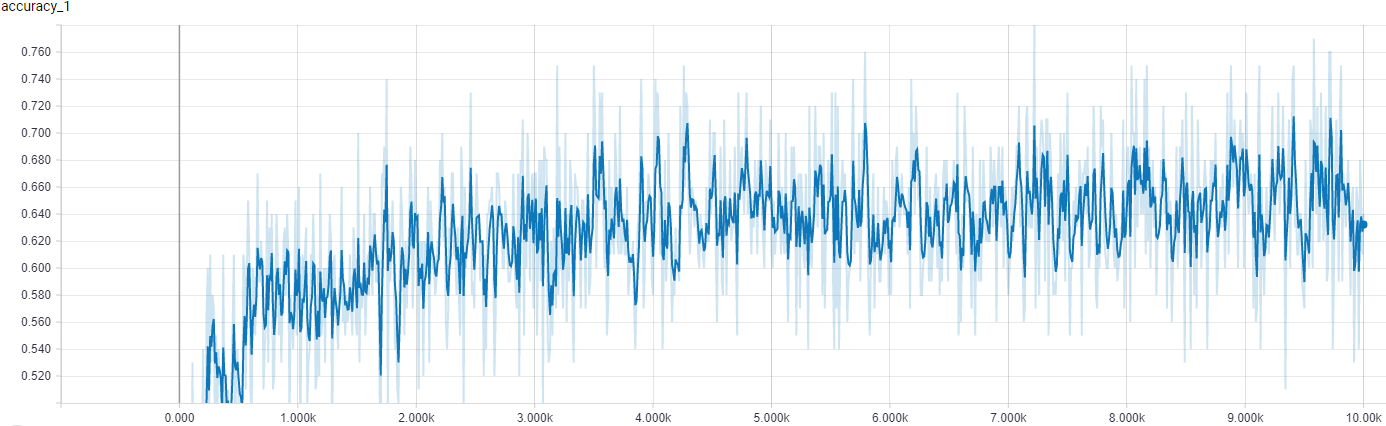
\includegraphics[scale=0.5]{model_val}
     \caption{Graph of accuracy of the validation dataset during training}
     \label{fig:model_train_val}
\end{figure}

\begin{figure}
    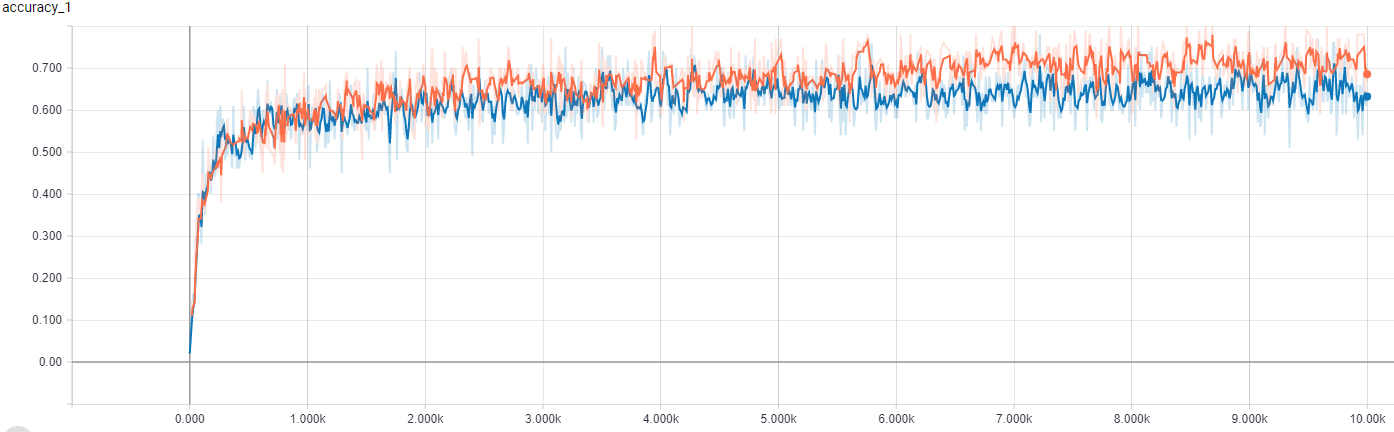
\includegraphics[scale=0.4]{test_val_accuracy}
     \caption{Comparison of accuracy}
     \label{fig:test_val_accuracy}
\end{figure}

\begin{figure}
    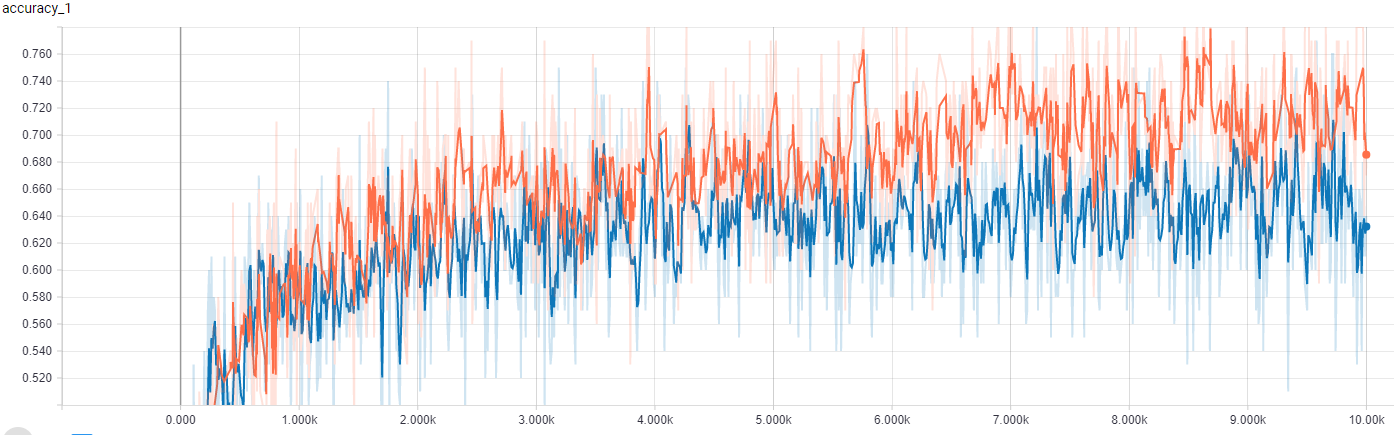
\includegraphics[scale=0.4]{test_val_accuracy_refined}
     \caption{Comparison of accuracy}
     \label{fig:test_val_accuracy_refined}
\end{figure}


\begin{table}[]
	\centering
	\caption{Comparison of parameters}
	\label{parameter_tuning_table}
	\begin{tabular}{llllll}
		Parameter Tuning & Steps & Learning Rate & Test \% & Validation \% &
		Results \\
		Configuration 1  & 8000  & default       & default & default       &
		59.1\%  \\
		Configuration 2  & 8000  & 0.1           & default & default       &
		65.8\%  \\
		Configuration 3  & 10000 & 0.1           & default & default       &
		66.3\%  \\
		Configuration 4  & 12000 & 0.1           & default & default       &
		66.6\%  \\
		Configuration 5  & 10000 & 0.2           & default & default       &
		66.0\%  \\
		Configuration 6  & 10000 & 0.1           & 15      & 15            &
		66.3\% 
	\end{tabular}
\end{table}

\subsection*{Empirical Analysis}
The results of each set of parameters can be seen in Table
\ref{parameter_tuning_table}. The set of parameters that seem to be the most
effective are 10000 steps with a 0.1 learning rate. Graphs of this model can be
see in Figures \ref{fig:model_train_val} and \ref{fig:model_train_test}. These
are based on the validation set and then the test set respectively. A side by
side comparision can also be seen in Figures \ref{fig:test_val_accuracy} and
\ref{fig:test_val_accuracy_refined} where orange is for during training and blue
for the validation set.
\subsection*{Analysis}
There were two separate factors that each increased classification accuracy of
about 5\% each. These were training steps and learning rate.

Training steps are related to the number of images so before, when the training
steps were at 4000, not all of our training images were being used. As the steps were increased
twofold we saw a 3.8\% increase in accuracy.

Another parameter that increased accuracy significantly was learning rate. The
default learning rate is 0.01 which I increased to 0.1. This resulted in an
increase of 6.7\%. This is most likely due to the fact that since we are only
looking at the last layer, we can afford to change the weights more
significantly.
